

\documentclass[11pt]{article}%
\usepackage{amsfonts}
\usepackage{amssymb}
\usepackage{graphicx}
\usepackage{setspace}
\usepackage[round]{natbib}
\usepackage{amsmath}%
\usepackage{amsthm}%
\usepackage{palatino}
\usepackage{paralist}
\usepackage{subcaption}
\usepackage{xcolor}
\usepackage{multirow}
\usepackage{booktabs}
\usepackage{dsfont}
\usepackage{indentfirst}
\usepackage{enumerate}
\usepackage{longtable}
\usepackage{caption}
\usepackage{algorithm}
\usepackage{algpseudocode} 

\usepackage{tikz}
\usetikzlibrary{arrows}
\usetikzlibrary{positioning}
\usetikzlibrary{calc}
\usetikzlibrary{positioning,arrows.meta}
\newdimen\nodeDist
\nodeDist=25mm

\usepackage[hyperindex,breaklinks]{hyperref}
\hypersetup{colorlinks=true,       % false: boxed links; true: colored links
	linkcolor=red,       
	citecolor=blue,        % color of links to bibliography
	filecolor=magenta,      % color of file links
	urlcolor=cyan           % color of external links
}  

\newcommand{\Var}{\text{Var}}
\newcommand{\Cov}{\text{Cov}}
\newcommand{\I}{\mathbf{I}}
\newcommand{\quantile}{\text{Quantile}}
\newcommand{\defeq}{\mathrel{\mathop:}=}
\newcommand{\Z}{\mathbf{Z}}
\newcommand{\Ztilde}{\mathbf{\tilde{Z}}}
\newcommand{\F}{\mathbf{F}}
\newcommand{\R}{\mathbf{R}}
\newcommand{\B}{\mathbf{B}}
\newcommand{\E}{\mathbf{E}}
\newcommand{\W}{\mathbf{W}}
\newcommand{\V}{\mathbf{V}}
\newcommand{\N}{\mathcal{N}}
\newcommand{\M}{\mathcal{M}}
\newcommand{\U}{\mathbf{U}}
\newcommand{\HH}{\mathbf{H}}
\newcommand{\rr}{\mathbf{r}}
\newcommand{\D}{\mathbf{D}}
\newcommand{\trans}{\text{trans}}
\newcommand{\Q}{\mathbf{Q}}
\newcommand{\BEL}{\textbf{BEL }}



\def\argmin{\operatornamewithlimits{arg\,min}}
\DeclareMathOperator{\iid}{\stackrel{\mbox{\tiny iid} }{\sim}}
\newcommand{\logit}{\mbox{logit}}
\newcommand{\bPsi}{\mathbf{\Psi}}
\newcommand{\bbeta}{\boldsymbol{\beta}}
\newcommand{\X}{\mathbf{X}}
\newcommand{\w}{\mathrm{w}}
\newcommand{\Y}{\tilde{Y}}
\newcommand{\tepsilon}{\tilde{\epsilon}}
\newcommand{\blambda}{\mathbf{\lambda}}
\newcommand{\br}{\mathbf{r}}
\newcommand{\bv}{\mathbf{b}}
\newcommand{\f}{\mathbf{f}}
\newcommand{\btheta}{\boldsymbol{\theta}}
\newcommand{\epsy}{\epsilon}
\newcommand{\epsz}{\nu}
\newcommand{\z}{\mathrm{z}}
\newcommand{\cc}{\mathbf{c}}
\newcommand{\y}{\mathrm{y}}
\newcommand{\bSigma}{\boldsymbol{\Sigma}}
\newcommand{\probit}{\mbox{probit}}
\newcommand{\hiw}{\mbox{{\small\textsc{HIW}}}}
\newcommand{\iw}{\mbox{{\small\textsc{IW}}}}
\newcommand{\T}{\mbox{{\small\textsc{T}}}}
\newcommand{\C}{\mbox{{\small\textsc{C}}}}
\newcommand{\Ga}{\mbox{{\small\textsc{Ga}}}}
\newcommand{\IG}{\mbox{{\small\textsc{IG}}}}
\newcommand{\Be}{\mbox{{\small\textsc{Be}}}}
\newcommand{\Ber}{\mbox{{\small\textsc{Ber}}}}
\newcommand{\dd}{\mbox{d}}
\newcommand{\res}{\mathrm{r}}
\newcommand{\Tau}{\mathrm{T}}
\newcommand{\x}{\mathbf{x}}
\newcommand{\sayan}[1] {{\textcolor{red}{ #1}}}
\newtheorem{theorem}{Theorem}
\newtheorem{claim}{Claim}
\newtheorem{proposition}{Proposition}
\newtheorem{lemma}{Lemma}
\newtheorem{corollary}{Corollary}
\newtheorem{assumption}{Assumption}
\newenvironment{example}[1][Example]{\begin{trivlist}
		\item[\hskip \labelsep {\bfseries #1}]}{\end{trivlist}}
\newenvironment{remark}[1][Remark]{\begin{trivlist}
		\item[\hskip \labelsep {\bfseries #1}]}{\end{trivlist}}
\newcommand\independent{\protect\mathpalette{\protect\independenT}{\perp}}
\def\independenT#1#2{\mathrel{\rlap{$#1#2$}\mkern2mu{#1#2}}}

\usepackage[toc,page]{appendix}

\usepackage{setspace}
\doublespacing

\bibliographystyle{chicago}

\setcounter{MaxMatrixCols}{10}
\textwidth=6.6in
\textheight=8.9in
\headheight=0.0in
\oddsidemargin=0.0in
\headsep=0.0in
\topmargin=0.0in
\setlength\parindent{24pt}


\setlength{\abovedisplayskip}{5pt}
\setlength{\belowdisplayskip}{5pt}

% xinhe tree plot
\usepackage{tikz}
\tikzset{
	treenode/.style = {shape=rectangle, 
		draw, align=center,
		top color=white, bottom color=white},
	env/.style      = {treenode}
}

\tikzstyle{level 1}=[level distance=3cm, sibling distance=12cm, font=\large]
\tikzstyle{level 2}=[level distance=3cm, sibling distance=6cm, font=\large]
\tikzstyle{level 3}=[level distance=3cm, sibling distance=3cm, font=\large]
\tikzstyle{level 4}=[level distance=3cm, sibling distance=1.5cm, font=\normalsize]
\tikzstyle{level 5}=[level distance=3cm, sibling distance=1cm, font=\small]
\tikzstyle{level 6}=[level distance=3cm, sibling distance=3cm, font=\footnotesize]
\tikzstyle{level 7}=[level distance=3cm, sibling distance=2cm, font=\footnotesize]
\tikzstyle{level 8}=[level distance=3cm, sibling distance=1cm, font=\scriptsize]
\usepackage[paperheight=14cm,paperwidth=25cm,margin=0cm,heightrounded]{geometry}


\begin{document}
	\thispagestyle{empty}
	
	\begin{figure}[t!]
		\centering
		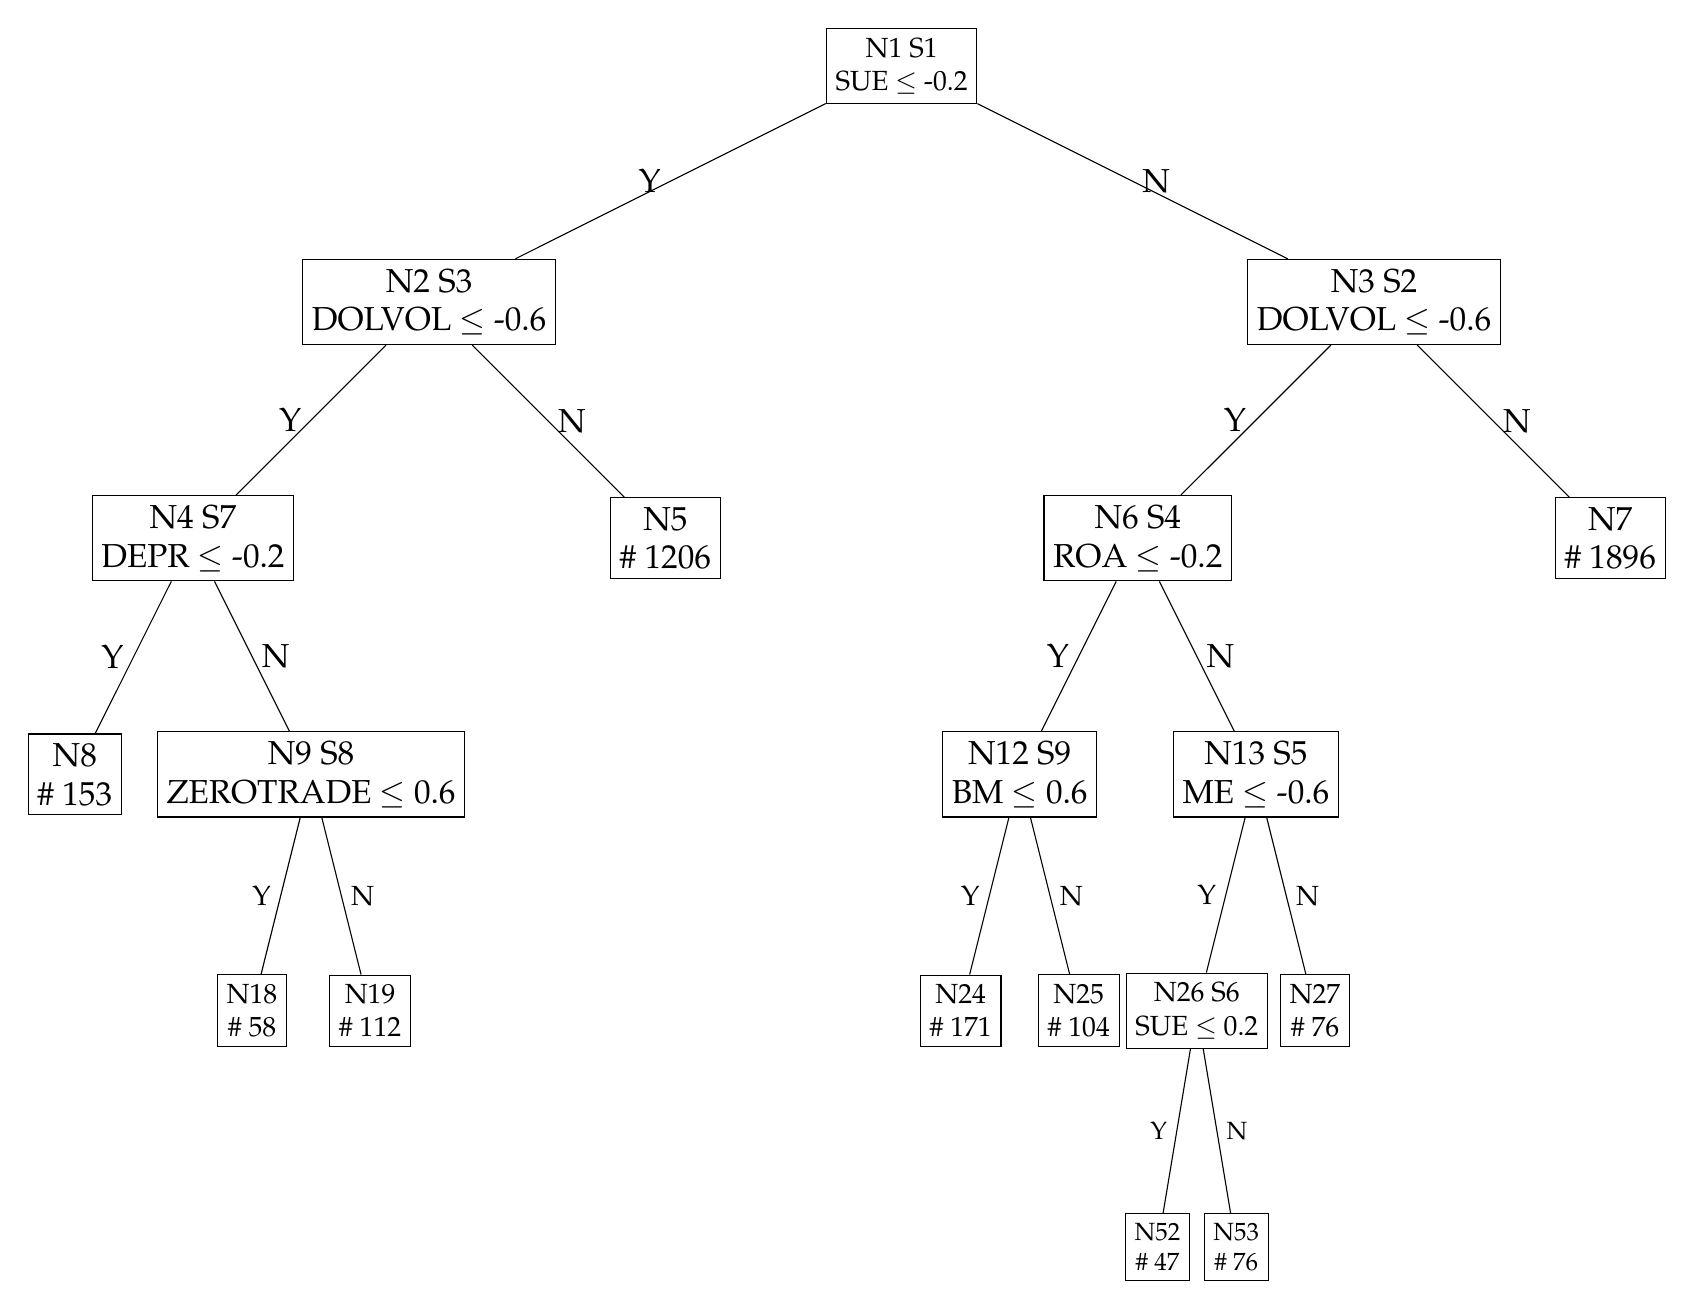
\begin{tikzpicture}
			[
			grow                    = down,
			edge from parent/.style = {draw},
			]			
%start python generated 
\node [env] {N1  S1\\ SUE $\leq$ -0.2 } 
      child { node [env] {N2  S3 \\ DOLVOL $\leq$ -0.6} 
            child { node [env] {N4  S7 \\ DEPR $\leq$ -0.2} 
                  child { node [env] {N8   \\ \# 153 } 
                        edge from parent node [left] {Y} 
                  }
                  child { node [env] {N9  S8 \\ ZEROTRADE $\leq$ 0.6} 
                        child { node [env] {N18   \\ \# 58 } 
                              edge from parent node [left] {Y} 
                        }
                        child { node [env] {N19   \\ \# 112 } 
                              edge from parent node [right] {N} 
                        }
                        edge from parent node [right] {N} 
                  }
                  edge from parent node [left] {Y} 
            }
            child { node [env] {N5   \\ \# 1206 } 
                  edge from parent node [right] {N} 
            }
            edge from parent node [left] {Y} 
      }
      child { node [env] {N3  S2 \\ DOLVOL $\leq$ -0.6} 
            child { node [env] {N6  S4 \\ ROA $\leq$ -0.2} 
                  child { node [env] {N12  S9 \\ BM $\leq$ 0.6} 
                        child { node [env] {N24   \\ \# 171 } 
                              edge from parent node [left] {Y} 
                        }
                        child { node [env] {N25   \\ \# 104 } 
                              edge from parent node [right] {N} 
                        }
                        edge from parent node [left] {Y} 
                  }
                  child { node [env] {N13  S5 \\ ME $\leq$ -0.6} 
                        child { node [env] {N26  S6 \\ SUE $\leq$ 0.2} 
                              child { node [env] {N52   \\ \# 47 } 
                                    edge from parent node [left] {Y} 
                              }
                              child { node [env] {N53   \\ \# 76 } 
                                    edge from parent node [right] {N} 
                              }
                              edge from parent node [left] {Y} 
                        }
                        child { node [env] {N27   \\ \# 76 } 
                              edge from parent node [right] {N} 
                        }
                        edge from parent node [right] {N} 
                  }
                  edge from parent node [left] {Y} 
            }
            child { node [env] {N7   \\ \# 1896 } 
                  edge from parent node [right] {N} 
            }
            edge from parent node [right] {N} 
      }

%end python generated 
;
		\end{tikzpicture}
	\end{figure}
	
	
	
\end{document}
